\begin{example}[Advection-diffusion 2D]
\label{ex:quart2}
Based on Example 2 \cite{Antonietti2013},
in $\Omega = \langle 0, 1 \rangle^2$ we will again solve equation \eqref{eq:ex_advdiff}
%\begin{equation}
%	\pdiff{u}{x} + \pdiff{u}{y} - D \cdot \left( \pdiff{^2 u}{x^2} + \pdiff{^2 
%	u}{y^2} \right) = g
%\end{equation}
%i.e
%\begin{equation}
%	\vec{a} \cdot \nabla u - D \Delta u = g
%\end{equation}
%where $\vec{a} = [1, 1]^T$ is advection velocity and $D$ is diffusion 
%coefficient and $g$ is a source function. 
We set up boundary condition and source function in such a way that the exact 
solution $u_{exact}$ is
\begin{equation}
	u_{exact} =  -\arctan\left(\frac{4 \, {\left(2 \, x - 1\right)}^{2} + 4 \, {\left(2 
	\, y - 1\right)}^{2} - 
	1}{16 \, \sqrt{\mathit{D}}}\right).
\end{equation}
We omit analytical forms of $g$ and boundary conditions for brevity, they can be found in 
the code. Different values of coefficient $C_w$ in penalty term yield different 
convergence behavior as demonstrated in Figure \ref{fig:conv_qart2} and 
\Cref{fig:orders_quarteroni2}. For very low values of diffusion coefficient $D$ the 
solution develops into cylinder. In this state high values of $C_w$ are detrimental as 
they prevent steep edges and cause artifacts in solution, for illustration compare 
\cref{fig:sol_quart2_a} and \cref{fig:sol_quart2_b} in (a) the relative error of 
approximate solution significantly less then in (b) despite visible discontinuities. 
Antonietti et al. \cite{Antonietti2013} report convergence for order 1 and 2, these are 
in accord with ours.

\end{example}
\begin{figure}[h!]
\centering
\begin{tabular}{p{0.5\textwidth} p{0.5\textwidth}}
	\vspace{0pt} 
	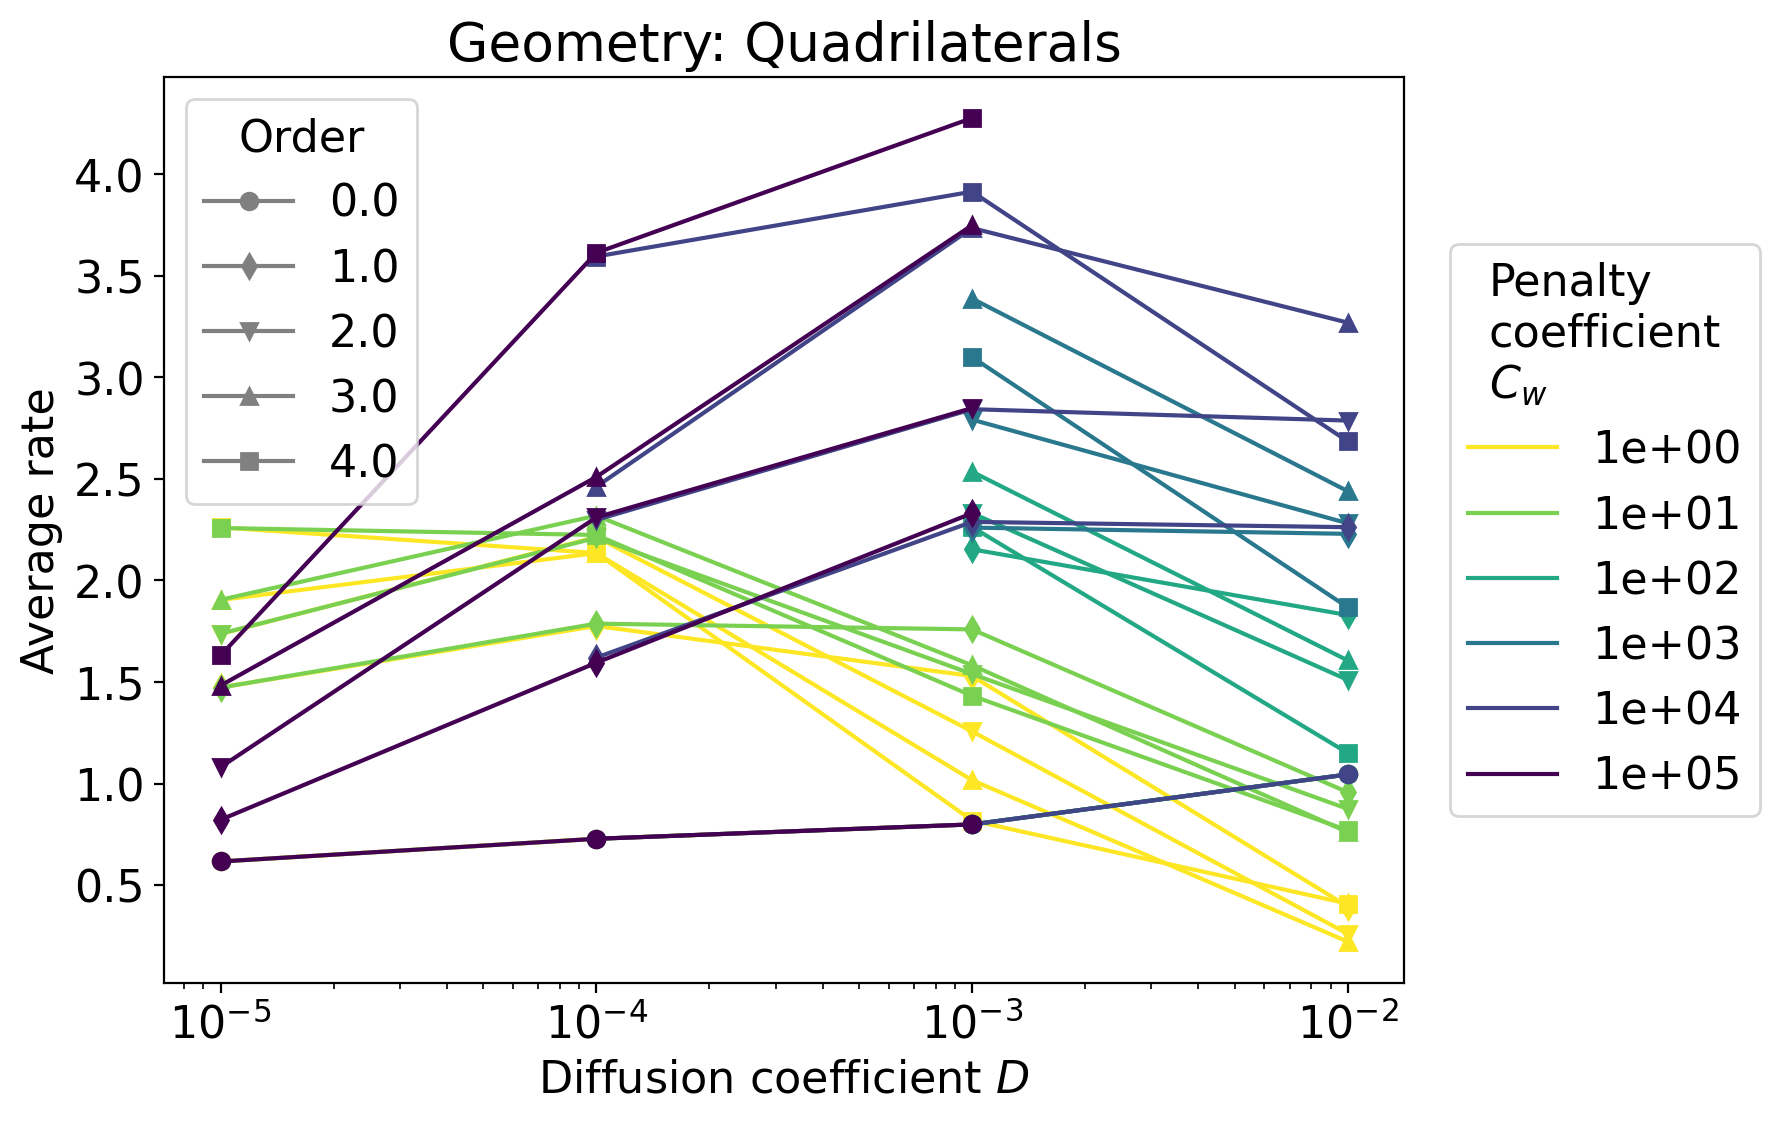
\includegraphics[width=0.4\textwidth]{../figs/parametric/advdiff_2D/ord_quarteroni2_2_4}
	&
	\vspace{0pt} 
	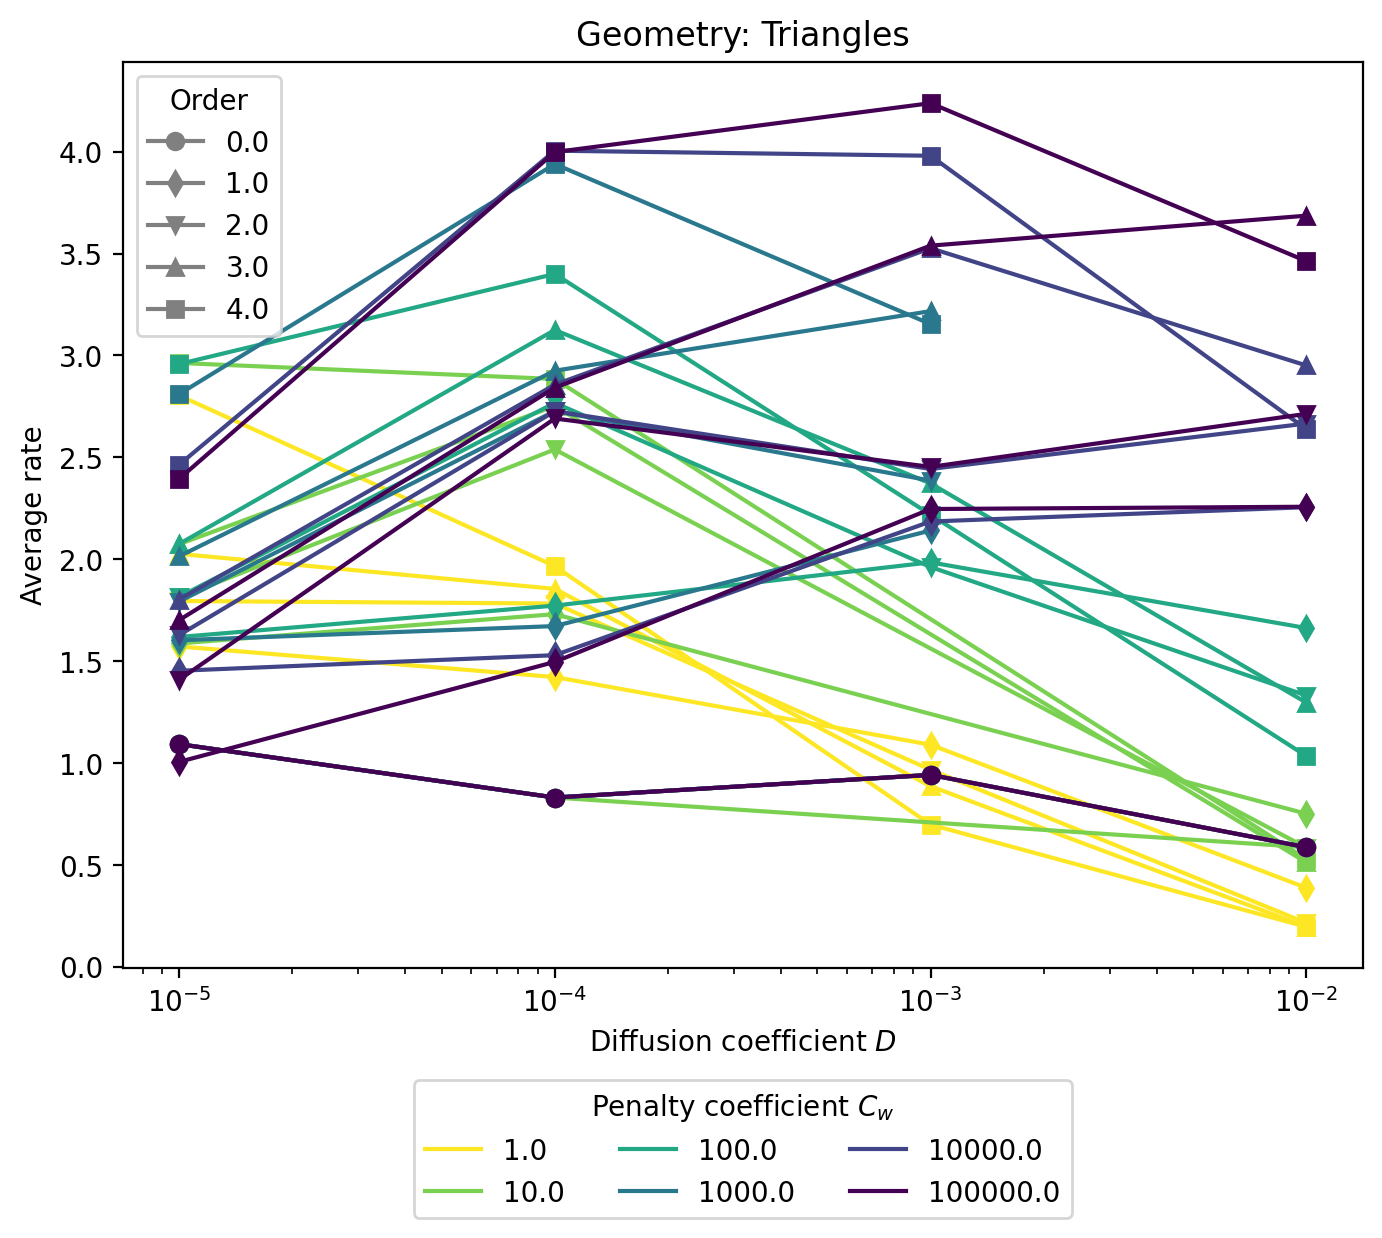
\includegraphics[width=0.4\textwidth]{../figs/parametric/advdiff_2D/ord_quarteroni2_2_3}
\end{tabular}
\caption{\Cref{ex:quart2}. Average convergence rate for different choices of $C_w$ for 
quadrilaterals (left) and triangles (right).}
\label{fig:orders_quarteroni2}
\end{figure}

\begin{figure}[h!]
    \centering
    \begin{subfigure}{.5\textwidth}	
        \centering	
        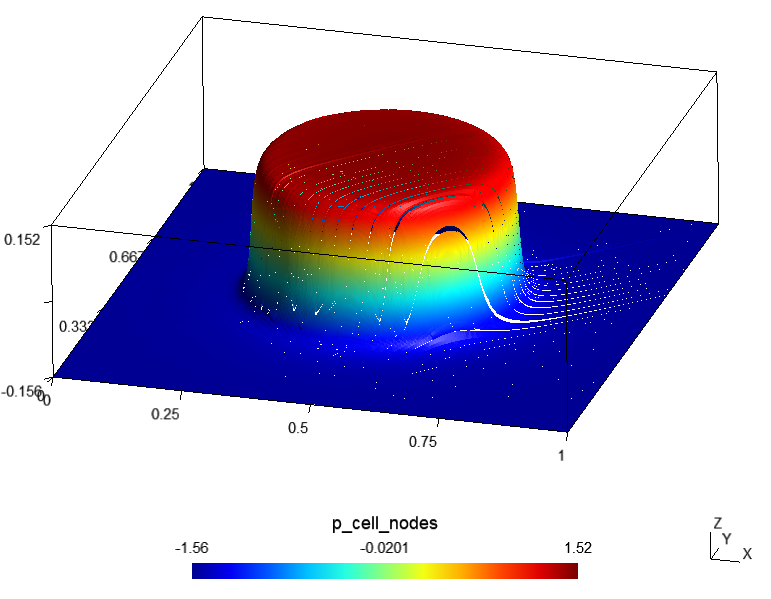
\includegraphics[width=\linewidth]{../figs/sols/quart2-0000000000010-sol-h4096o04}
        \caption{$C_w = 1$}
        \label{fig:sol_quart2_a}
    \end{subfigure}%
    \begin{subfigure}{.5\textwidth}
        \centering	
        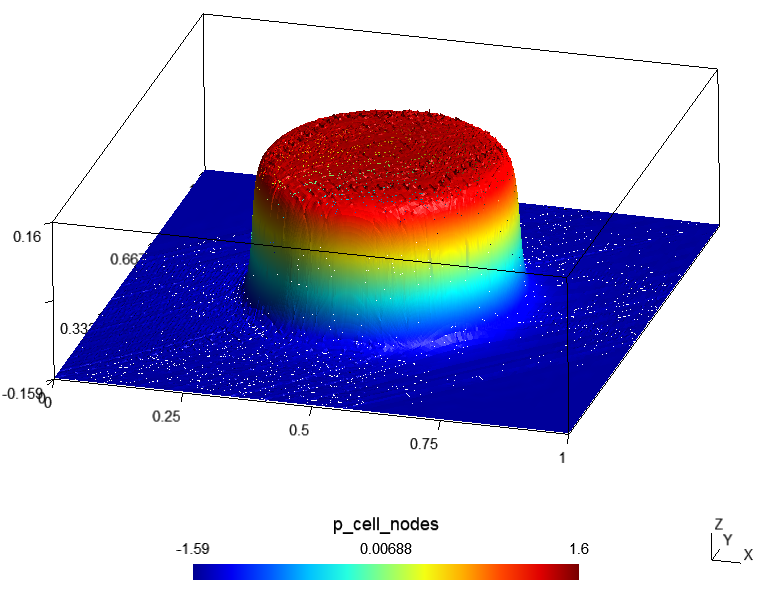
\includegraphics[width=\linewidth]{../figs/sols/quart2-0005000000010-sol-h4096o04}
        \caption{$C_w = 10^5$}
        \label{fig:sol_quart2_b}
    \end{subfigure}
    \caption{\Cref{ex:quart2}. Solutions for $D = 10^{-5}$, on triangular mesh with 
    $4096$ elements, 4th order approximation. The visualization was scaled 
    down by factor $0.1$ in vertical axis.}
    \label{fig:sol_quart2}
\end{figure}


\begin{figure}[p!]
	\centering
	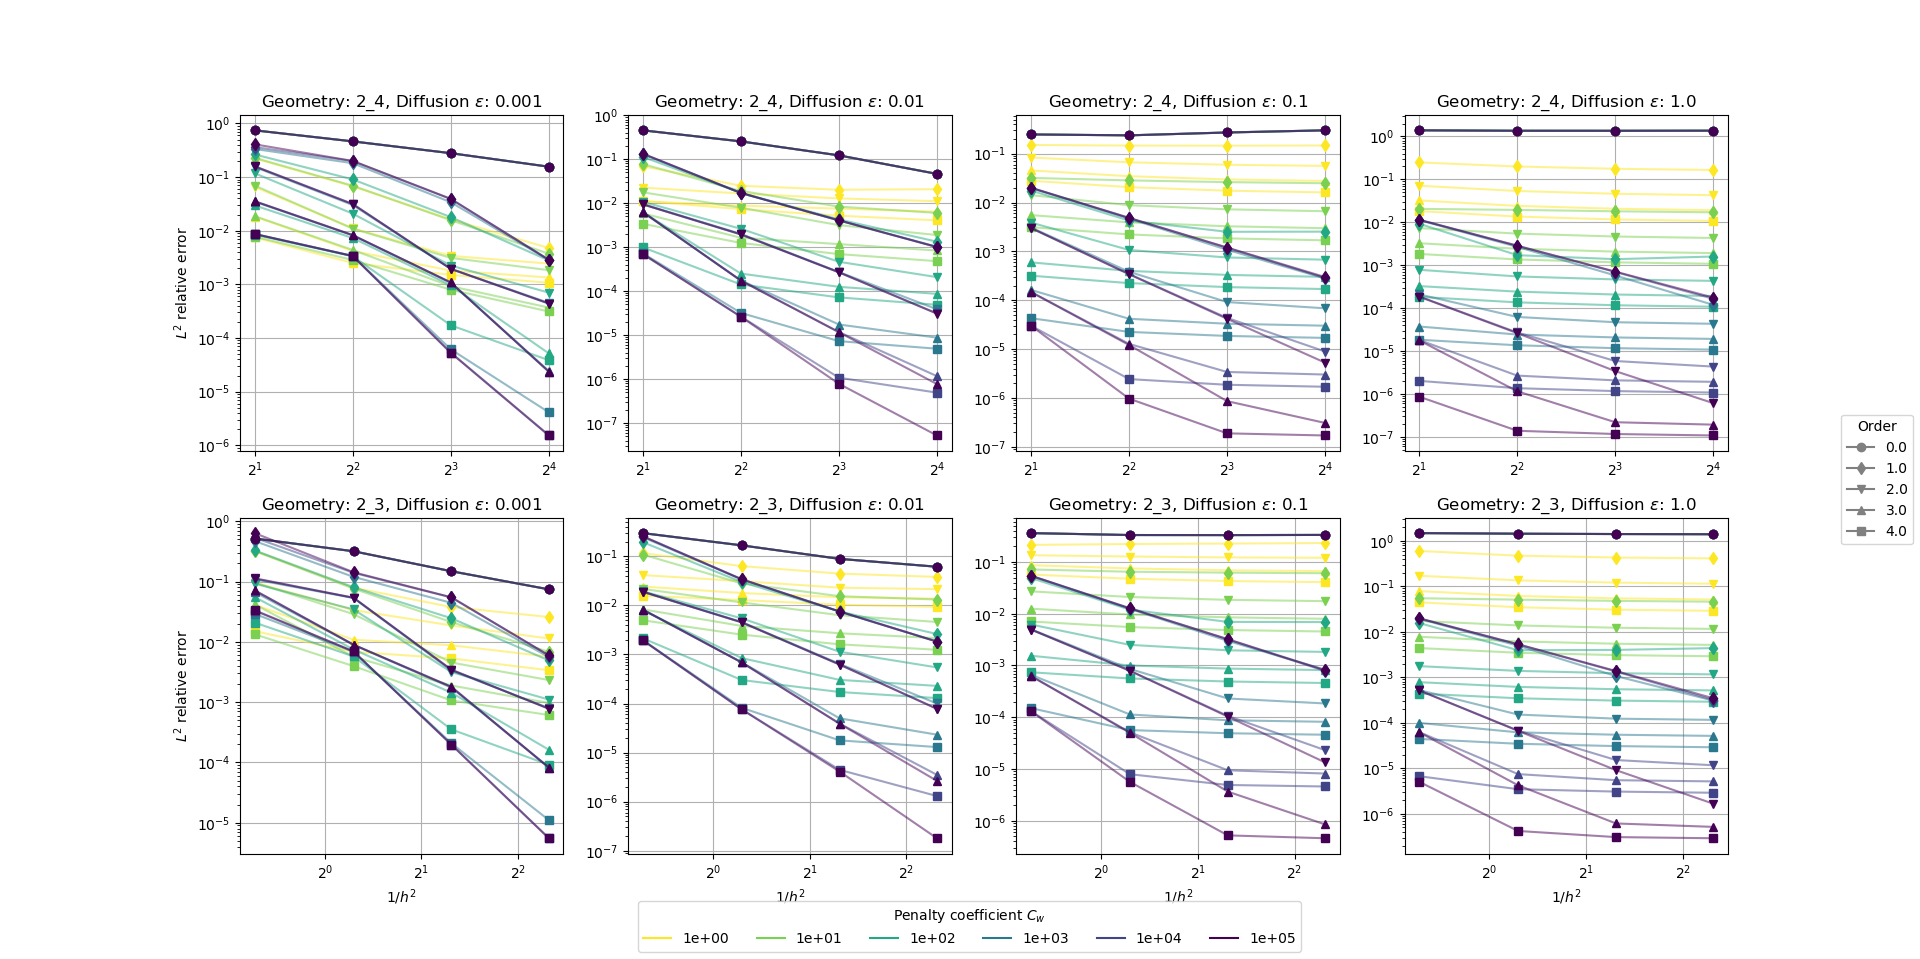
\includegraphics[height=\textheight]{../figs/parametric/advdiff_2D/quarteroni2.png}
	\caption{\Cref{ex:quart2}. Relative errors for different choices of $C_w$ for 
	quadrilaterals (left) and triangles (right).}
	\label{fig:conv_qart2}
\end{figure}

